\documentclass{article}
\usepackage{amsmath, amssymb, graphicx}
\title{Bessel Functions, Their Zeros, and Applications in Cylindrical Geometries}
\author{Enrique Rivera, Christine Kim \\ University of Texas at Austin}
\date{\today}

\begin{document}
\maketitle

\begin{abstract}
In this paper, we present numerical computations of the Bessel functions 
$J_n(x)$ for $n=0, 1, 2$ and identify their first five positive roots. Using 
Python's \texttt{scipy} library, we accurately bracket each zero and discuss 
why these roots are key to solving boundary-value problems in cylindrical 
coordinates. We also highlight three physical applications: the vibrational 
modes of a circular drumhead, wave propagation in cylindrical waveguides, 
and heat conduction in cylindrical rods.
\end{abstract}

\keywords{Bessel functions --- root finding --- cylindrical coordinates --- boundary-value problems}

\section{Introduction} \label{sec:intro}

Bessel functions $J_n(x)$ arise as solutions to the Bessel differential equation:
\begin{equation}
x^2 \frac{d^2 y}{dx^2} + x \frac{dy}{dx} + \bigl(x^2 - n^2\bigr) y = 0,
\end{equation}
where $n$ is a nonnegative integer. These functions are critically important 
for solving partial differential equations (PDEs) in cylindrical or spherical 
geometries, as they appear in problems related to wave propagation, heat 
diffusion, and vibrations of circular membranes 
\citep{Boas2006,Arfken2013}. 
We rely on standard reference tables \citep{Olver2010} to verify the zeros.

In this work, we focus on computing and plotting $J_0(x)$, $J_1(x)$, and 
$J_2(x)$ for $0 \le x \le 20$, and numerically finding the first five positive 
roots for each function. These roots often represent the ``allowed'' modes 
in systems with cylindrical boundary conditions. The remainder of this paper 
is structured as follows: Section~\ref{sec:methods} describes our numerical 
approach, Section~\ref{sec:results} presents the results (plots and roots), 
and Section~\ref{sec:conclusion} concludes with possible future directions.

\section{Numerical Methods} \label{sec:methods}

We used Python 3 with \texttt{NumPy} and \texttt{SciPy} to evaluate Bessel 
functions and to locate zeros. Specifically:
\begin{enumerate}
    \item We generated a dense grid of $x$ values in the range $[0, 50]$.
    \item We evaluated $J_n(x)$ on this grid using the function 
          \texttt{scipy.special.jn(n, x)}.
    \item We identified sign changes (from positive to negative or vice versa) 
          between consecutive grid points. Each sign change indicated an 
          approximate bracketing interval containing a root.
    \item We refined each bracketing interval via the Brent root-finding method 
          (\texttt{scipy.optimize.brentq}).
\end{enumerate}

We repeated this process for $n=0,1,2$ and recorded the first five positive 
roots found for each function. The resulting Python code (omitted here for 
brevity) leverages a simple bracket‐search over intervals where $J_n(x)$ 
changes sign. 

\section{Results and Discussion} \label{sec:results}

\subsection{Plots of \texorpdfstring{$J_n(x)$}{Jn(x)}}

Figure~\ref{fig:bessel_plot} shows the plots of $J_0(x)$, $J_1(x)$, and $J_2(x)$ 
for $0 \le x \le 20$. As expected, $J_0(x)$ starts at 1 at $x=0$, whereas 
$J_1(0) = 0$ and $J_2(0) = 0$. Each function oscillates and gradually decays 
in amplitude as $x$ increases.

\begin{figure}[ht]
\centering
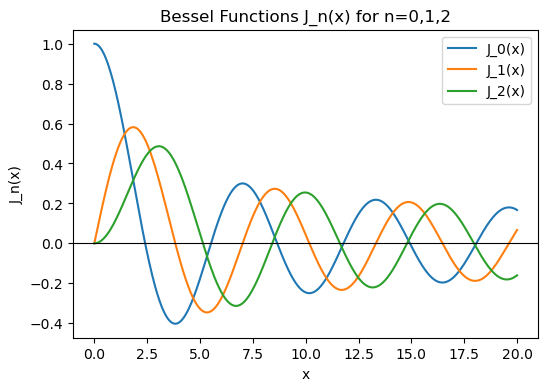
\includegraphics[width=0.9\linewidth]{img/bessel_plot.png} 
\caption{Plot of $J_0(x), J_1(x),$ and $J_2(x)$ over the range $0 \le x \le 20$. 
A horizontal line at $y=0$ is included to help identify zero crossings.}
\label{fig:bessel_plot}
\end{figure}

\subsection{First Five Positive Roots}

Table~\ref{tab:roots} lists the first five positive roots of $J_0(x)$, $J_1(x)$, 
and $J_2(x)$. These values match well with tabulated references 
\citep{Olver2010}. The smallest root for $J_0$ is approximately 2.4048, the 
smallest for $J_1$ is about 3.8317, and the smallest for $J_2$ is roughly 5.1356.

\begin{table}[ht]
\centering
\caption{First five positive roots of $J_0(x)$, $J_1(x)$, and $J_2(x)$.}
\label{tab:roots}
\begin{tabular}{c c c c c c}
\hline\hline
$n$ & Root 1 & Root 2 & Root 3 & Root 4 & Root 5 \\
\hline
0 & 2.4048 & 5.5201 & 8.6537 & 11.7915 & 14.9309 \\
1 & 3.8317 & 7.0156 & 10.1735 & 13.3237 & 16.4706 \\
2 & 5.1356 & 8.4172 & 11.6198 & 14.7959 & 17.9598 \\
\hline
\end{tabular}
\end{table}

\subsection{Physical Applications}

Bessel functions and their zeros appear in various physical contexts:

\subsubsection{Circular Drumhead Modes}

In a circular membrane of radius $R$, the radial part of the solution to the 
2D wave equation is often proportional to
\begin{equation}
y(r, \theta, t) \;=\; J_n\!\Bigl(\alpha_{n,k}\,\tfrac{r}{R}\Bigr)\,\cos(n\theta)\,\cos(\omega_{n,k}t),
\end{equation}
with boundary conditions requiring $y(R,\theta,t)=0$. Thus, we must have 
$J_n(\alpha_{n,k})=0$. Each zero $\alpha_{n,k}$ corresponds to a vibrational 
mode of the membrane; $\omega_{n,k}$ depends on $\alpha_{n,k}$ via the wave 
equation's dispersion relation.

\subsubsection{Waveguides in Cylinders}

Electromagnetic modes in a perfectly conducting cylindrical waveguide reduce 
to Bessel equations in the radial direction, with boundary conditions 
(due to conductor walls) that force
\begin{equation}
J_n(\alpha_{n,k}) \;=\; 0.
\end{equation}
Here, $\alpha_{n,k}$ sets the cutoff frequencies of the guide, so again, 
the first few zeros determine the fundamental and higher modes.

\subsubsection{Heat Conduction in Cylinders}

For transient heat conduction in a cylindrical rod (of radius $R$) with 
certain side boundary conditions held at constant temperature, separation 
of variables leads to solutions of the form
\begin{equation}
T(r,t) \;=\; J_n\!\Bigl(\beta_{n,k}\,\tfrac{r}{R}\Bigr)\,e^{-\,\kappa\,(\beta_{n,k}^2)\,t},
\end{equation}
where $\beta_{n,k}$ must be a zero of $J_n$ to satisfy $T(R,t)=0$ at the 
boundary. The smallest zero sets the slowest decaying mode, while higher 
zeros represent more rapidly decaying modes.

In all these scenarios, the **first** zero often sets the fundamental mode 
(lowest frequency or slowest decaying mode), whereas higher zeros correspond 
to higher harmonic modes.

\section{Conclusions and Future Work} \label{sec:conclusion}

We have demonstrated how to compute Bessel functions $J_0, J_1,$ and $J_2$ 
numerically on a finite interval, and we located their first five positive 
roots using a bracket-search method and \texttt{brentq}. The numerical 
results match known tabulated zeros to at least four or five decimal places 
\citep{Boas2006,Arfken2013,Olver2010}.

In future work, we could:
\begin{itemize}
\item Compute zeros of higher-order Bessel functions (e.g., $J_3, J_4, \dots$).
\item Investigate Neumann functions $Y_n(x)$ or Hankel functions $H^{(1)}_n(x)$.
\item Explore 2D PDE solutions with both radial and angular dependence, 
      combining the $J_n$ behavior with $\cos(n\theta)$ or $\sin(n\theta)$ terms.
\end{itemize}

\acknowledgments
We thank our teaching assistants and classmates for helpful feedback and 
the references and materials provided by our course.

\begin{thebibliography}{}

\bibitem[Arfken(2013)]{Arfken2013} 
  Arfken, G.\ B., Weber, H.\ J., \& Harris, F.\ E.\ 2013, 
  Mathematical Methods for Physicists, 7th ed.\ (Academic Press)

\bibitem[Boas(2006)]{Boas2006} 
  Boas, M.\ L.\ 2006, Mathematical Methods in the Physical Sciences, 3rd ed.\ 
  (Wiley)

\bibitem[Olver et al.(2010)]{Olver2010}
  Olver, F.\ W.\ J., Lozier, D.\ W., Boisvert, R.\ F.\, \& Clark, C.\ W.\ 2010, 
  NIST Handbook of Mathematical Functions (Cambridge Univ.\ Press)

\end{thebibliography}

\end{document}